\chapter{Evaluation and Interpretation}
\label{ch:viz}

While the previous chapter focuses on algorithmic uses of topic
models, one of the reasons for using topic models is that they produce
human-readable summaries of the themes of large document collections.  However,
for users to use the results of topic models, they must be able to understand
the models' output.  This depends on model \emph{visualization},
\emph{interaction}, and \emph{evaluation}.

We begin this chapter with a discussion of how best to show individual
topics to users.  From these foundations, we move to how we can
display entire models---with many topics---to users.  Finally, we
close with how users can provide feedback through these interfaces to
detect errors and improve the underlying model.

\section{Displaying Topics}
\label{sec:display}

Recall from the previous chapters that topics are distributions over words; the
words with the highest weight in a topic best explain what the topic is about.
While the simplest answer---just show the most probable words---is a common
solution, there are possible refinements that can improve a user's understanding
of a collection by showing the relationships between words or explicitly showing
words' probability.

% cite TACL paper
\paragraph{Word Lists}

Just showing a list of the most common words (a
visualization that we will call ``word list'') is very simple, and it also works well.
Users can quickly understand how words are arranged, and it is an efficient use of
space. 
Topics have been represented horizontally~\citep{gardner2010topic,smith2015visual} or
vertically~\citep{eisenstein2012topicviz,chaney2012visualizing}, with or without
commas separating the individual words, or using set
notation~\citep{chaney2012visualizing}.  \citet{smith2015visual} go further by
adding bars representing the probabilities of the word.

\paragraph{Word Clouds}

\begin{figure}
  \begin{center}
    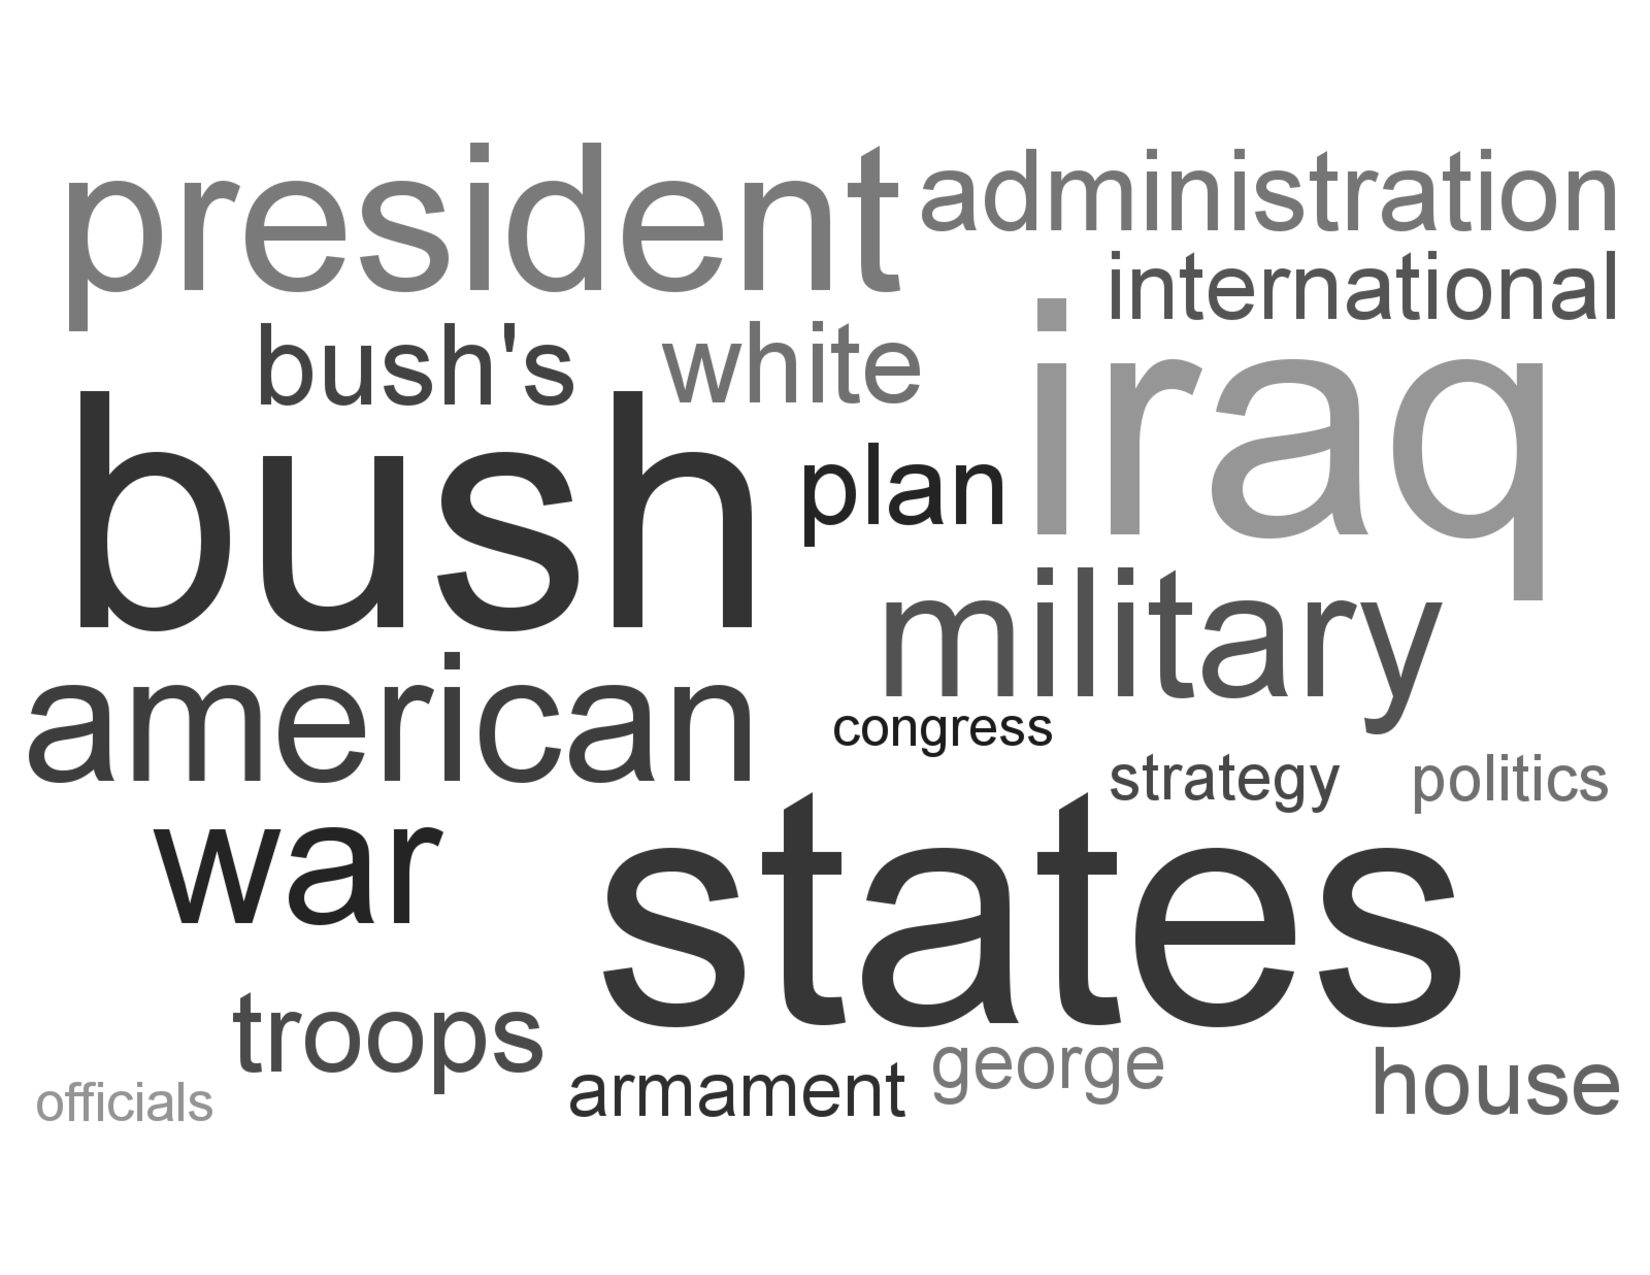
\includegraphics[width=.5\linewidth]{figures/wordcloud_20}
  \end{center}
  \caption{Word clouds use a 2D layout to show which words appear in a
  topic.  Word size is related to its probability in the topic,
  showing which words are more prominent.}
  \label{fig:word-cloud}
\end{figure}

Word clouds (e.g., Figure~\ref{fig:word-cloud}) are another popular approach for
displaying topics.  Unlike word lists, they also use the size of words to convey
additional information. Word clouds typically use the size of words to reflect
the probability of the words.  This uses more of a given visualization area to
be used to display a topic.

\begin{figure}
  \begin{center}
    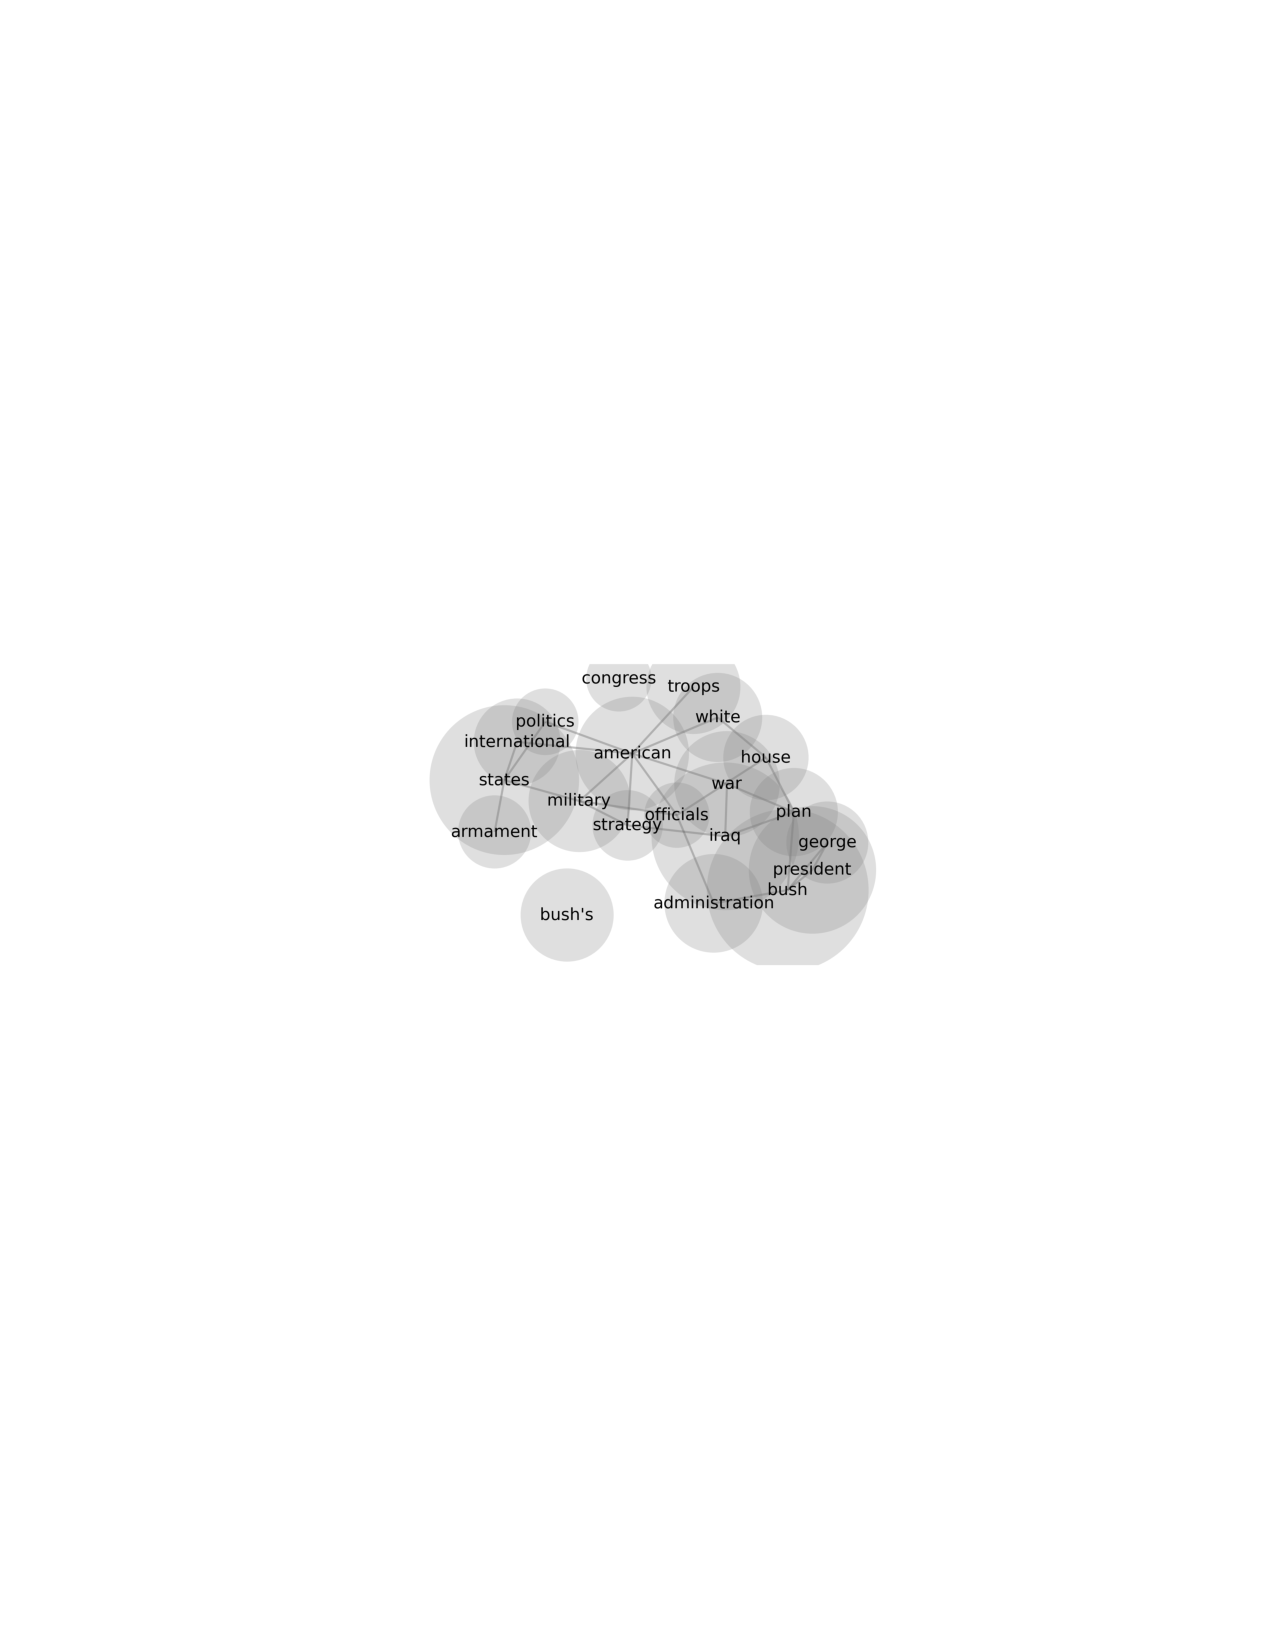
\includegraphics[width=.5\linewidth]{figures/topic_in_a_box_20}
  \end{center}
  \caption{A topic-in-a-box visualization for topics---like a word
    cloud---shows words in a 2D context.  However, it uses local
    co-occurence (whether words appear together in a sentence) to decide which words to place next to each other.}
  \label{fig:topic-in-a-box}
\end{figure}

However, word clouds have been criticized for providing poor support for visual
search~\citep{Viegas2008} and lacking contextual information between
words~\citep{harris11}; users can sometimes draw false connections between words
that are placed next to each other randomly in a word cloud.  Another
alternative is to use word associations to set the position of
words~\citep{Smith:Chuang:Hu:Boyd-Graber:Findlater-2014};
Figure~\ref{fig:topic-in-a-box} places words that appear together next to
each other in the visualization.

% \subsection{When Words aren't Enough}

% Multi-word expressions can be discovered through
% pre-processing~\citep{talley-11}, post-processing step~\citep{blei-09b},
% or a joint model~\citep{johnson-10}.

\section{Labeling Topics}

\index{topic labeling}
Throughout this survey, we have been referring to topics with \emph{labels} such as
\underline{information technology} or \underline{the arts}.  These are
convenient descriptors, but completely removed from the raw distribution over words.
Thus, it is often useful to assign labels to topics within an interface.

In contrast to the previous \emph{visualization} approaches, labeling
focuses on showing not the original words of a topic but rather a
clearer label more akin to what a human summary of the data would
provide.

Approaches for automatic labeling can be divided into those that only
use internal information from the topic model against those that also
use external knowledge resources.  While purely internal methods are
more robust and consistent with the philosophy of unsupervised topic
models, external resources often produce higher quality
labels.

Of the techniques that use external resources, we further separate
those that use direct supervision for labeling (i.e., knowing what
constitutes a good labeling) from those that use general knowledge
resources such as Wikipedia or knowledge bases.

\paragraph{Internal Labeling}

\citet{mei-07} propose an internal labeling method that takes
prominent phrases from the topic and compares how consistent the
phrase's context is with the topic distribution.  Phrases whose
contexts closely resemble the topic often appear in regions of text
that summarize the document, making them good candidates for labels.
\citet{mao-12} extend the technique to hierarchies, using the insight
that parents' labels should be consistent with their children's.

% What about Tim W at UIUC?

% I didn't really understand this paper: Automatic Labelling of Topic
% Models Learned from Twitter by Summarisation (shoud we cite?)

\paragraph{Labeling with Supervised Labels}

% Frank Wood / Noemi hierarchically supervised model?

\citet{lau-10} use a supervised approach to rerank the words in a
topic to ensure that the ``best'' word in the topic is shown to a
user. Each candidate word forms a feature vector consisting of
features such as the following:
\begin{itemize*}
\item the conditional probability of a word given the other words in a
  topic (which implies topic coherence, as discussed in
Chapter~\ref{sec:coherence});
\item whether the word is a hypernym of other words in the topic
  (e.g., ``dog'' in a topic that also contains ``terrier'' and
  ``poodle''); and
\item the original probability of the word in the topic.
\end{itemize*}

\index{Wikipedia}
While these can be used alone as an unsupervised reranking,
\citet{lau-10} use user-selected best topic words to weight which of
these features are most important for selecting the best topic word.
These weights are learned using support vector regression.
\citet{lau-11} extend their technique by adding candidates from
Wikipedia to the set.
The weakness of this approach is that Wikipedia may not have coverage
of the topics in the collection; if Wikipedia ignores the theme
captured by a topic model, then it will fail to find an appropriate
label for that topic.

\paragraph{Labeling with Knowledge Bases}

% Perhaps have a figure to give an example
\citet{mao-12} align topic models with an external ontology of labels.
They argue that labels should match topic words (as labeling with flat
topics); a topic's words should be consistent with a labels' children
in the hierarchy; and the topic's labels should be unique.

\index{PageRank}
\citet{aleteras-14} instead query the whole Web and then build a graph that
includes the words that make up the titles of the retrieved webpages. 
Their goal is to find words that are ``central'' in the graph: these
words should make for a good title.
Words have edges between them if they appear close to each other more
than one would expect by chance.
This property is measures through the  the normalized pointwise mutual
information (\abr{npmi}) metric.
They find the central words by using the PageRank~\citep{page-99}
algorithm, which finds words that are highly probable in the topic and appear frequently
with many other words in the topic.
This is the same algorithm that search engines use to find pages that
have ``high authority'' on the Internet.

Just like a search engine should return \texttt{simpsonsarchive.com}
for a search on ``the Simpsons'' because everyone links to it, this
labeling method will find the word in a topic that all of the other
words ``vote for''.  
For each word in a topic, we find all of the
words that are likely to also appear with that word and then take the
winner of that election as our label for a topic.  For example, given
the topic
\begin{quote}
cell response immune lymphocyte antigen cytokine t-cell induce
receptor immunity
\end{quote}
the algorithm selects \underline{immune system}, as it appears near many of
the other terms in the topic~\citep{aleteras-14}.

\paragraph{Using Labeled Documents}

\index{labeled \abr{lda}}
The task of associating labels with topics becomes much easier if many of your
documents are themselves labeled.  Labeled \abr{lda}~\citep{ramage-09}
associates topics to each of the labels and forces labeled documents to only use
the topics associated with the document.  This constraint forces the topics to
be consistent with the original labels (Figure~\ref{fig:llda}).
\citet{Bakalov-12} extend this to hierarchical label sets (e.g., \abr{ny} Times
subjects that place \underline{Russia} under \underline{International}), while
\citet{nguyen:boyd-graber:resnik:chang-2014} extend it to learning hierarchies
of topics from unorganized labels, learning that \underline{ska}\footnote{A musical genre, familiar to reggae fans and cruciverbalists.} is a
kind of \underline{music} without provided links.

\begin{figure}
  \begin{center}
    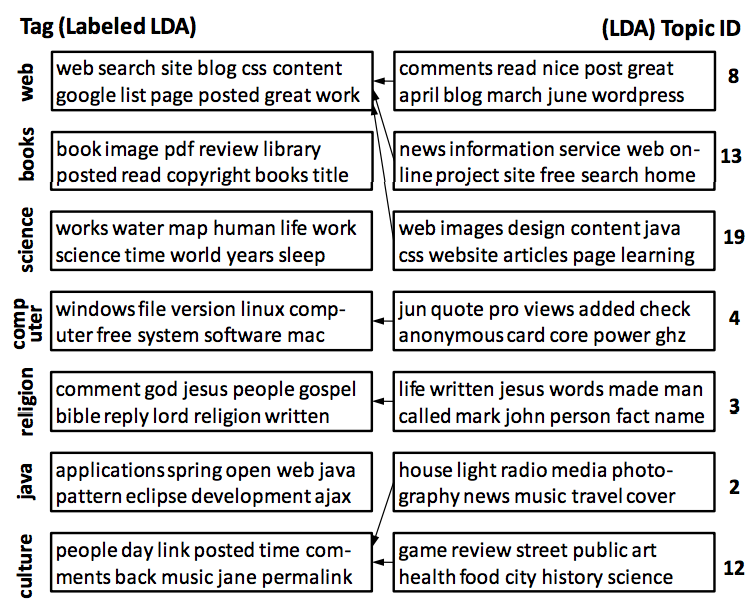
\includegraphics[width=.7\linewidth]{figures/viz_llda}
  \end{center}
  \caption{Example of topics learned by labeled \abr{lda} (Figure from
    \citet{ramage-09}).  Each topic in labeled \abr{lda} is associated with a
    label, which encourages the topics to be consistent with the ontology of
    labels.  \abr{lda}, in contrast, uses the empirical frequency of topics to
    divide the collection, resulting in three topics (8, 13, 19) associated with
    the labeled \abr{lda} \underline{web} topic. }
  \label{fig:llda}
\end{figure}


\section{Displaying Models}

\begin{figure}
  \begin{center}
  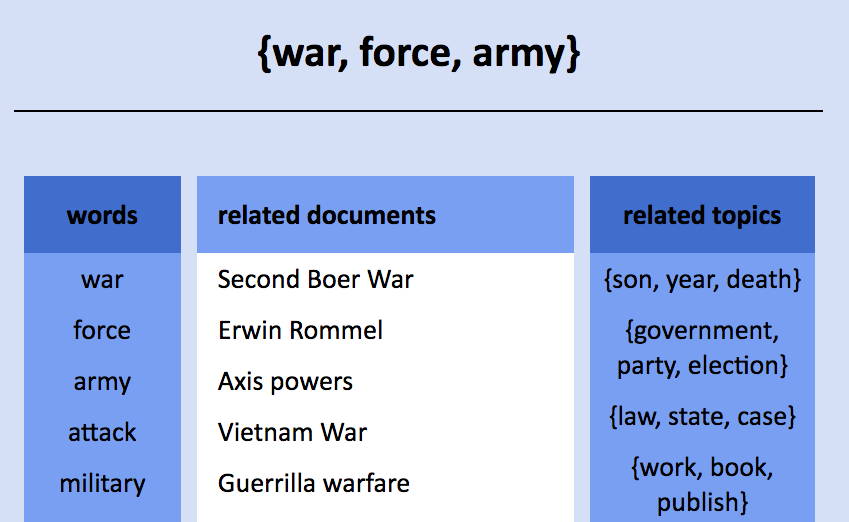
\includegraphics[width=.8\linewidth]{figures/viz_tmve}
  \end{center}
  \caption{The Topic Model Visualization Engine~\citep{chaney-12}
    shows the most related documents to a topic along with related topics. }
  \label{fig:tmve}
\end{figure}

However, topics are not the end of the story.  Users often want to use topics to
find relevant documents within the collection.  Going back to our
example in a
previous chapter, a user may want to find the ``smoking gun'' in the Enron
corpus, not just use topics to understand the main themes in a collection.

\index{topic model visualization engine}
Thus, a good topic model visualization must also show the documents associated
with a topic.  The Topic Model Visualization Engine~\citep[\abr{tmve}]{chaney-12} shows the
top documents associated with a topic (Figure~\ref{fig:tmve}).  Recall that each
document has a distribution over topics~$\theta_d$, which is a vector with an
entry for each topic.  We focus on the dimension associated with a particular topic
and then sort the documents based on that topic coordinate from largest to
smallest.

\index{topical guide}
The topical guide~\citep{gardner-10} extends this approach by enriching topic
views with additional metadata.  For instance, if the collection has dollar
amounts or sentiment~\citep{pang-08} associated with a document, it provides a
histogram of the metadata associated with the topic.  It also provides \emph{in
  context} examples of topic words, allowing to see how a word is used within a
topic (helping to address the topic model's bag of words assumptions).

\index{interactive topic model and metadata}
Interactive TOpic Model and MEtadata~\citep[Interactive TOpic Model and MEtadata]{eistenstein-14} focuses on a specific type of metadata: time.
It allows users to view the evolution of topics over time to understand, for
example, how the issue of slavery is reframed from an economic argument to an
argument over human rights.  It supports filtering to specific topics or to see
how words are used over time across topics.

\abr{termite}
Rather than showing how topics relate to metadata,
\citet{chuang-12} focus on how topics relate to \emph{each other}.
Their ``Termite'' topic visualization (Figure~\ref{fig:termite}) shows
the term-by-term similarity between topics.  By presenting topic-term
probabilities on a grid with topics as the columns and terms as the
rows, users can see when topics share words or when topics are only
about a handful of words.

\begin{figure}
  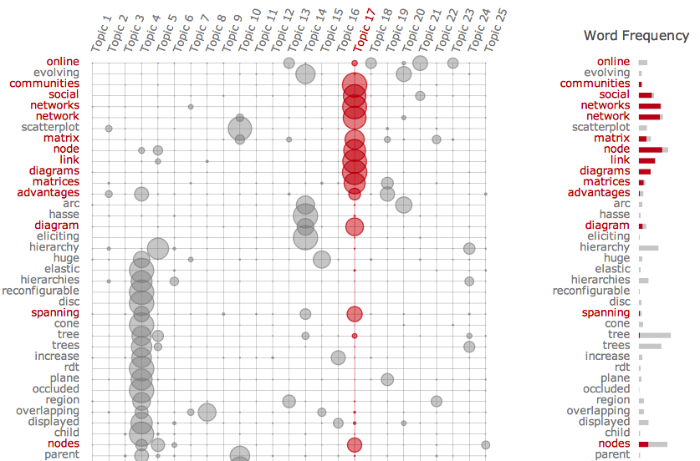
\includegraphics[width=.9\linewidth]{figures/viz_termite}
  \caption{The Termite visualization of topics helps reveal which
    topics use similar words and are thus likely talking about similar
    things.}
  \label{fig:termite}
\end{figure}

\section{Evaluation, Stability, and Repair}
\label{sec:coherence}

Visualizations can help show users where topic models have issues.
Topic models are rarely perfect, and quality can vary within a
model. Even in good models we often find several poorly fit or
improperly combined topics. 

\index{likelihood evaluation}
For many years, the primary metric for evaluating the quality of a
topic model was the held-out likelihood of a model~\citep{wallach-09a}.
Because a topic model is a generative probabilistic model---like a
language model~\citep{chen-98}---we can ask how well the model can
predict unseen text: run the generative process forward for the
document and see how well that matches up with the held-out document.
If the model does a good job of using topics to predict what words
will appear in new documents, then it is a good model, and if it fails
to do so, it is a bad model.

In some ways held-out likelihood makes sense, but it is incomplete.
We should be able to detect some kinds of failure: topics that are just random noise will have poor held-out likelihood.
On the other hand, it is possible to get good held-out likelihood with a large set of topics so specific that any held-out document is modeled well.
The topics would nevertheless lack generalizability and interpretability.

\citet{chang-09b} show that
held-out likelihood, a traditional measure of probabilistic model quality,
emphasizes \emph{complexity} rather than the ease of interpretability
that users are looking for.  
User ratings of how good topics negatively correlate with
held-out likelihood: a more complex model (e.g., a model with more
complicated equations or a model with more topics) can better fit a random
held-out document. 
More complex models, however, are more confusing for users. 

\index{topic coherence}
Automated measurements~\citep{newman-10,mimno-11,lau-14} of topic
quality may serve as a proxy for human interpretability ratings.
However, these approaches may not be able to tell you
whether a topic model is suitable for a specific application, which parts of a model are reliable, or why.
Showing the relationships between multiple models can also help
distinguish stable from spurious topics~\citep{chuang-15}, and
adjusting the ``hyperparameters'' of distributions (the Dirichlet
parameters of models discussed in Chapter~\ref{ch:intro}) can have a
large effect of what the final models are~\citep{wallach-09b}.

\citet{tang-14} provide a diagnosis manual for what properties of a
dataset can cause the failure of a topic model: a mismatch between the
number of topics and documents, topics that are ``too close
together'', or a mismatch between the number of topics in a document
and the Dirichlet parameter~$\alpha$.

\begin{figure}

\begin{minipage}[b]{0.4\textwidth}
\begin{tabular}{p{.9\textwidth}}
	Topic Words (before) \\ \hline \red{bladder}, sci,
        \blue{spinal\_cord}, \blue{spinal\_cord\_injury},
        \blue{spinal}, \red{urinary}, \red{urinary\_tract},
        \red{urothelial},\blue{injury}, \blue{motor}, \blue{recovery},
        \blue{reflex}, \blue{cervical}, \red{urothelium},
        \blue{functional\_recovery} \\
\end{tabular}
\end{minipage}
  \hfill
\begin{minipage}[b]{0.4\textwidth}
\begin{tabular}{p{.9\textwidth}}
	Topic Words (after) \\ \hline sci, \blue{spinal\_cord},
        \blue{spinal\_cord\_injury}, \blue{spinal}, \blue{injury},
        \blue{recovery}, \blue{motor}, \blue{reflex},
        \red{urothelial}, \green{injured},
        \blue{functional\_recovery}, \green{plasticity},
        \green{locomotor}, \blue{cervical}, \green{locomotion}\\
\end{tabular}
\end{minipage}

\caption{Example topics before and after interactive topic modeling from
  \citet{hu-14:itm}.  Initially, the topic conflates two topics
  (\red{urinary} and \blue{central nervous system}), which is undesirable.  Adding
a constraint that the words ``bladder'' and ``spinal cord'' should not
appear together in a topic makes the topic more coherent and discovers
concepts that \green{were not present before}.}
\label{fig:itm-nih}
\end{figure}

\index{interactivity!topic models}
Interactive topic modeling---in conjunction with visualizations---can help
correct the problems of topic models.  A user first gets an overview of the
collection using a visualization of the topics and documents and can then
see and correct instances where the model makes mistakes.

For example, Figure~\ref{fig:itm-nih} shows a topic learned from abstracts of
grants funded by the American National Institutes of Health
(\abr{nih}, discussed more in Chapter~\ref{sec:sci_fields}).  Most
topics were ``good'': they summarized the data and told a story about
a coherent slice of research supported by the \abr{nih}.  However,
this topic is more problematic; it combines words about the central
nervous system with words about the urinary system.  Such a topic (as
discussed in \citet{mimno-11}) does not give a clear understanding of the
documents it should represent.

\citet{hu-14:itm} address this problem by allowing a user to add probabilistic
constraints to the model~\citep{boyd-graber-07,andrzejewski-09}.  For example,
the user might say that ``bladder'' and ``spinal cord'' do not belong in the same
topic together.  Figure~\ref{fig:itm-nih} shows how the topic is more focused after the
user provides this feedback.  In contrast to probabilistic constraints,
\citet{choo-13} and \citet{lund-17} use matrix factorization constraints to guide changes
to topics, which can be much faster.

\section{Summary}

While topic models provide users with overviews of corpora, topic models
cannot be much help if the users cannot effectively see or understand
the underlying topics and how they relate to specific documents.
Evaluations help to identify which portions of a model to trust and which to use with caution.
Interactive visualizations allow users to discover and
refine insights. In the next chapters we will talk about specific applications of
these insights, but these insights are often built on the initial understanding
of a model offered by the visualizations discussed in this chapter.
